\documentclass[11pt,a4paper]{report}

\usepackage[utf8]{inputenc}
\usepackage[margin=1in]{geometry}
\usepackage{amsmath,amssymb}
\usepackage{graphicx}
\usepackage{booktabs}
\usepackage{tabularx}
\usepackage{listings}
\usepackage{xcolor}
\usepackage{hyperref}
\usepackage{fancyhdr}
\usepackage{titlesec}
\usepackage{microtype}
\usepackage{caption}
\usepackage{subcaption}
\usepackage{cite}
\usepackage{float}
\usepackage{url}

% Color definitions
\definecolor{buetblue}{RGB}{0, 43, 73}
\definecolor{darkred}{RGB}{178, 34, 34}
\definecolor{codegreen}{RGB}{46, 139, 87}
\definecolor{codegray}{RGB}{100, 100, 100}
\definecolor{codebackground}{RGB}{248, 249, 250}
\definecolor{keywordblue}{RGB}{0, 51, 153}
\definecolor{linkblue}{RGB}{0, 70, 140}

% Hyperref setup
\hypersetup{
    colorlinks=true,
    linkcolor=linkblue,
    citecolor=linkblue,
    urlcolor=linkblue,
    pdftitle={CSE 406 Design Report: Topic 06 - TCP SYN Flood Attack and Defense},
    pdfauthor={Shahriar Ahmed Seam, Hozifa Rahman Hamim}
}

% Listings setup
\lstdefinestyle{customc}{
    backgroundcolor=\color{codebackground},
    commentstyle=\color{codegreen}\itshape,
    keywordstyle=\color{keywordblue}\bfseries,
    numberstyle=\tiny\color{codegray},
    stringstyle=\color{darkred},
    basicstyle=\ttfamily\footnotesize,
    breakatwhitespace=false,
    breaklines=true,
    captionpos=b,
    keepspaces=true,
    numbers=left,
    numbersep=6pt,
    showspaces=false,
    showstringspaces=false,
    showtabs=false,
    tabsize=4,
    frame=single,
    rulecolor=\color{black!20}
}

\lstdefinestyle{terminal}{
    backgroundcolor=\color{black!90},
    basicstyle=\ttfamily\footnotesize\color{green!80!white},
    breaklines=true,
    frame=single,
    rulecolor=\color{black},
    numbers=none
}

% Header and Footer
\pagestyle{fancy}
\fancyhf{}
\setlength{\headheight}{15pt}
\fancyhead[L]{\slshape \nouppercase{\leftmark}}
\fancyhead[R]{\thepage}
\fancyfoot{}
\renewcommand{\headrulewidth}{0.4pt}
\renewcommand{\footrulewidth}{0pt}

% Title Formatting & Continuous Flow
\titleclass{\chapter}{straight}
\titleformat{\chapter}[hang]
  {\normalfont\Large\bfseries\color{buetblue}}{\chaptertitlename\ \thechapter:}{8pt}{\Large}
\titlespacing*{\chapter}{0pt}{20pt plus 4pt minus 2pt}{10pt plus 2pt minus 2pt}
\titlespacing*{\section}{0pt}{14pt plus 2pt minus 2pt}{5pt}
\titlespacing*{\subsection}{0pt}{10pt plus 2pt minus 2pt}{3pt}

% Table formatting helper
\newcolumntype{Y}{>{\centering\arraybackslash}X}
\setlength{\textfloatsep}{10pt plus 2pt minus 2pt}
\setlength{\intextsep}{10pt plus 2pt minus 2pt}

\begin{document}

% =========================================================================
% COVER PAGE
% =========================================================================
\begin{titlepage}
    \centering
    \vspace*{1.5cm}
    
    {\Large \textbf{Bangladesh University of Engineering and Technology}}\\[0.35cm]
    {\large \textbf{Department of Computer Science and Engineering}}\\[2.2cm]
    
    {\Large \textbf{CSE 406: Computer Security Sessional}}\\[2.2cm]
    
    \rule{\linewidth}{0.5mm}\\[0.7cm]
    {\Large \bfseries TCP SYN Flood + DoS Attack and Defense Mechanisms}\\[0.7cm]
    \rule{\linewidth}{0.5mm}\\[2.5cm]
    
    {\large \textbf{Submitted By:}}\\[0.8cm]
    \begin{minipage}{0.45\textwidth}
        \centering \large
        \textbf{Shahriar Ahmed Seam}\\[0.15cm]
        Student ID: 2005093
    \end{minipage}
    \hfill
    \begin{minipage}{0.45\textwidth}
        \centering \large
        \textbf{Hozifa Rahman Hamim}\\[0.15cm]
        Student ID: 1705083
    \end{minipage}
    
    \vfill
    {\large \today}\\[0.8cm]
\end{titlepage}

% =========================================================================
% FRONT MATTER
% =========================================================================
\pagenumbering{roman}

\begin{abstract}
The Transmission Control Protocol (TCP, RFC 793) provides reliable, ordered data delivery across the Internet. To synchronize sequence numbers and establish communication parameters, TCP relies on a three-way handshake (SYN $\to$ SYN-ACK $\to$ ACK). This design introduces an asymmetry in resource allocation: an initiating client commits negligible local memory when transmitting a 40-byte SYN packet, whereas the receiving server must allocate kernel memory for a Transmission Control Block (TCB, tracked as \texttt{request\_sock} in Linux) and maintain an entry in its bounded SYN backlog queue.

In this project, we analyze, implement, and experimentally evaluate a \textbf{TCP SYN Flood Denial of Service (DoS) attack tool} written from scratch in standard C using low-level POSIX raw sockets (\texttt{SOCK\_RAW} with \texttt{IP\_HDRINCL}). In compliance with course policies, we did not use any third-party attack frameworks or packet-crafting libraries. We manually synthesized Layer 3 (IPv4) headers and Layer 4 (TCP) headers, implemented the RFC 1071 16-bit one's complement checksum routine with TCP pseudo-headers, and built a packet injection loop capable of delivering over $388,000$ packets per second.

We evaluated this implementation inside an isolated virtual network testbed to observe server degradation and test countermeasures. Under default conditions with defenses disabled (\texttt{tcp\_syncookies=0}), the attack exhausted the server's backlog queue within $25.6\text{ ms}$, driving legitimate connection timeout failure rates to $100\%$. To address the project bonus requirement, we implemented and evaluated four defensive layers: (1) Cryptographic Stateless TCP SYN Cookies (\texttt{tcp\_syncookies=1}), which removed server-side state allocation for initial requests and restored legitimate client success rates to $90\text{--}100\%$ during an active flood; (2) Ingress Firewall Rate Limiting using Netfilter \texttt{iptables}, which dropped $84.7\%$ of attack packets before they reached the socket queue; (3) Stateful Netfilter \texttt{SYNPROXY} connection handling; and (4) Kernel Parameter Hardening via \texttt{sysctl}. All experimental claims are supported by captured terminal traces, socket queue telemetry (\texttt{ss}, \texttt{netstat}), and measured client latency data.
\end{abstract}

% Front matter lists
\tableofcontents
\vspace{0.8cm}
\begingroup
\let\clearpage\relax
\listoffigures
\vspace{0.8cm}
\listoftables
\endgroup
\clearpage

\pagenumbering{arabic}

% =========================================================================
% CHAPTER 1: INTRODUCTION
% =========================================================================
\chapter{Introduction}

\section{Background and Motivation}
Most network services rely on the Transmission Control Protocol (TCP) to deliver reliable, sequenced, and error-checked byte streams over packet-switched networks. Common network applications, including web servers (HTTP/HTTPS), remote shells (SSH), database engines, and backend microservices, establish transport sessions through the standard three-way handshake defined in RFC 793.

Because connection establishment requires the server to maintain state before the client has verified its reachability, TCP services remain vulnerable to transport-layer Denial of Service (DoS) attacks. Among these, the \textbf{TCP SYN Flood} remains one of the oldest and most persistent attack vectors. By exploiting the server's obligation to reserve memory before the handshake completes, an attacker with modest network resources can exhaust connection tables and render high-capacity servers inaccessible to legitimate users.

\section{Problem Statement}
When a TCP server receives a synchronization segment ($SYN$), it creates an internal half-open connection record and responds with a synchronization-acknowledgment ($SYN\text{-}ACK$), waiting for the client's final acknowledgment ($ACK$). In a SYN flood attack, the adversary transmits a stream of $SYN$ packets carrying spoofed source IP addresses. Because these addresses point to non-existent, inactive, or unreachable hosts, the expected $ACK$ packet is never returned.

The server retains these half-open connection records in a bounded queue—known as the SYN backlog queue—and repeatedly retransmits $SYN\text{-}ACK$ packets according to an exponential backoff schedule. Under default Linux settings, this retention period lasts approximately 63 seconds. If spoofed requests arrive faster than expired half-open sockets are removed, the backlog queue fills completely. Once saturated, the operating system kernel discards incoming connection requests, denying access to all legitimate clients.

\section{Project Objectives and Scope}
This project was carried out under the specifications of Topic 06 for CSE 406. The primary technical objectives were:
\begin{enumerate}
    \item \textbf{Custom Attack Tool Implementation:} Build a standalone, high-rate TCP SYN flood injector in standard C using POSIX raw sockets (\texttt{AF\_INET}, \texttt{SOCK\_RAW}, \texttt{IPPROTO\_RAW}). Third-party attack tools (such as \texttt{hping3}, \texttt{Scapy}, or \texttt{nping}) were strictly excluded.
    \item \textbf{Bitwise Protocol Header Serialization:} Manually construct Layer 3 (IPv4) and Layer 4 (TCP) binary headers, implement random source IP and port generation, and implement RFC 1071 16-bit one's complement checksums using RFC 793 TCP pseudo-headers.
    \item \textbf{Isolated Testbed Deployment:} Build a multi-node virtual test environment comprising an Attacker Node, a Victim Web Server, a Legitimate Client, and an interconnecting virtual bridge to isolate all spoofed traffic from production networks.
    \item \textbf{Empirical Vulnerability Verification:} Experimentally record socket queue saturation, kernel drop telemetry (\texttt{ss}, \texttt{netstat}), and legitimate connection success and failure rates during attack activity.
    \item \textbf{Defensive Countermeasure Evaluation (Bonus Credit):} Implement, configure, and benchmark four defensive mechanisms: Cryptographic Stateless TCP SYN Cookies, Netfilter \texttt{iptables} ingress rate limiting, Netfilter \texttt{SYNPROXY}, and kernel parameter tuning.
\end{enumerate}

\section{Report Organization}
The remainder of this report is organized into ten chapters and one appendix:
\begin{itemize}
    \item Chapter 2 explains the theoretical mechanics of the TCP state machine, resource asymmetry, and IP address spoofing.
    \item Chapter 3 describes the virtual network testbed topology, node configurations, and kernel baselines.
    \item Chapter 4 develops the timing model and mathematical queue saturation derivation.
    \item Chapter 5 documents the bitwise frame, IPv4, and TCP header layouts.
    \item Chapter 6 reviews the C implementation details of \texttt{syn\_flood.c} and checksum calculations.
    \item Chapter 7 presents the empirical attack measurements, backlog exhaustion data, and client denial traces.
    \item Chapter 8 details the four implemented defenses and evaluates their performance under active flood conditions.
    \item Chapter 9 provides a comparative evaluation matrix and discusses security versus usability trade-offs.
    \item Chapter 10 summarizes the group work division and implementation milestones.
    \item Chapter 11 concludes the report and identifies avenues for future work.
    \item Appendix A provides project repository references and reproduction commands.
\end{itemize}

% =========================================================================
% CHAPTER 2: THEORETICAL BACKGROUND
% =========================================================================
\chapter{Theoretical Background \& Protocol Mechanics}

\section{The TCP State Machine and Three-Way Handshake}
Under RFC 793, TCP establishes a bidirectional byte stream between two endpoints by synchronizing initial sequence numbers:

\begin{figure}[H]
    \centering
    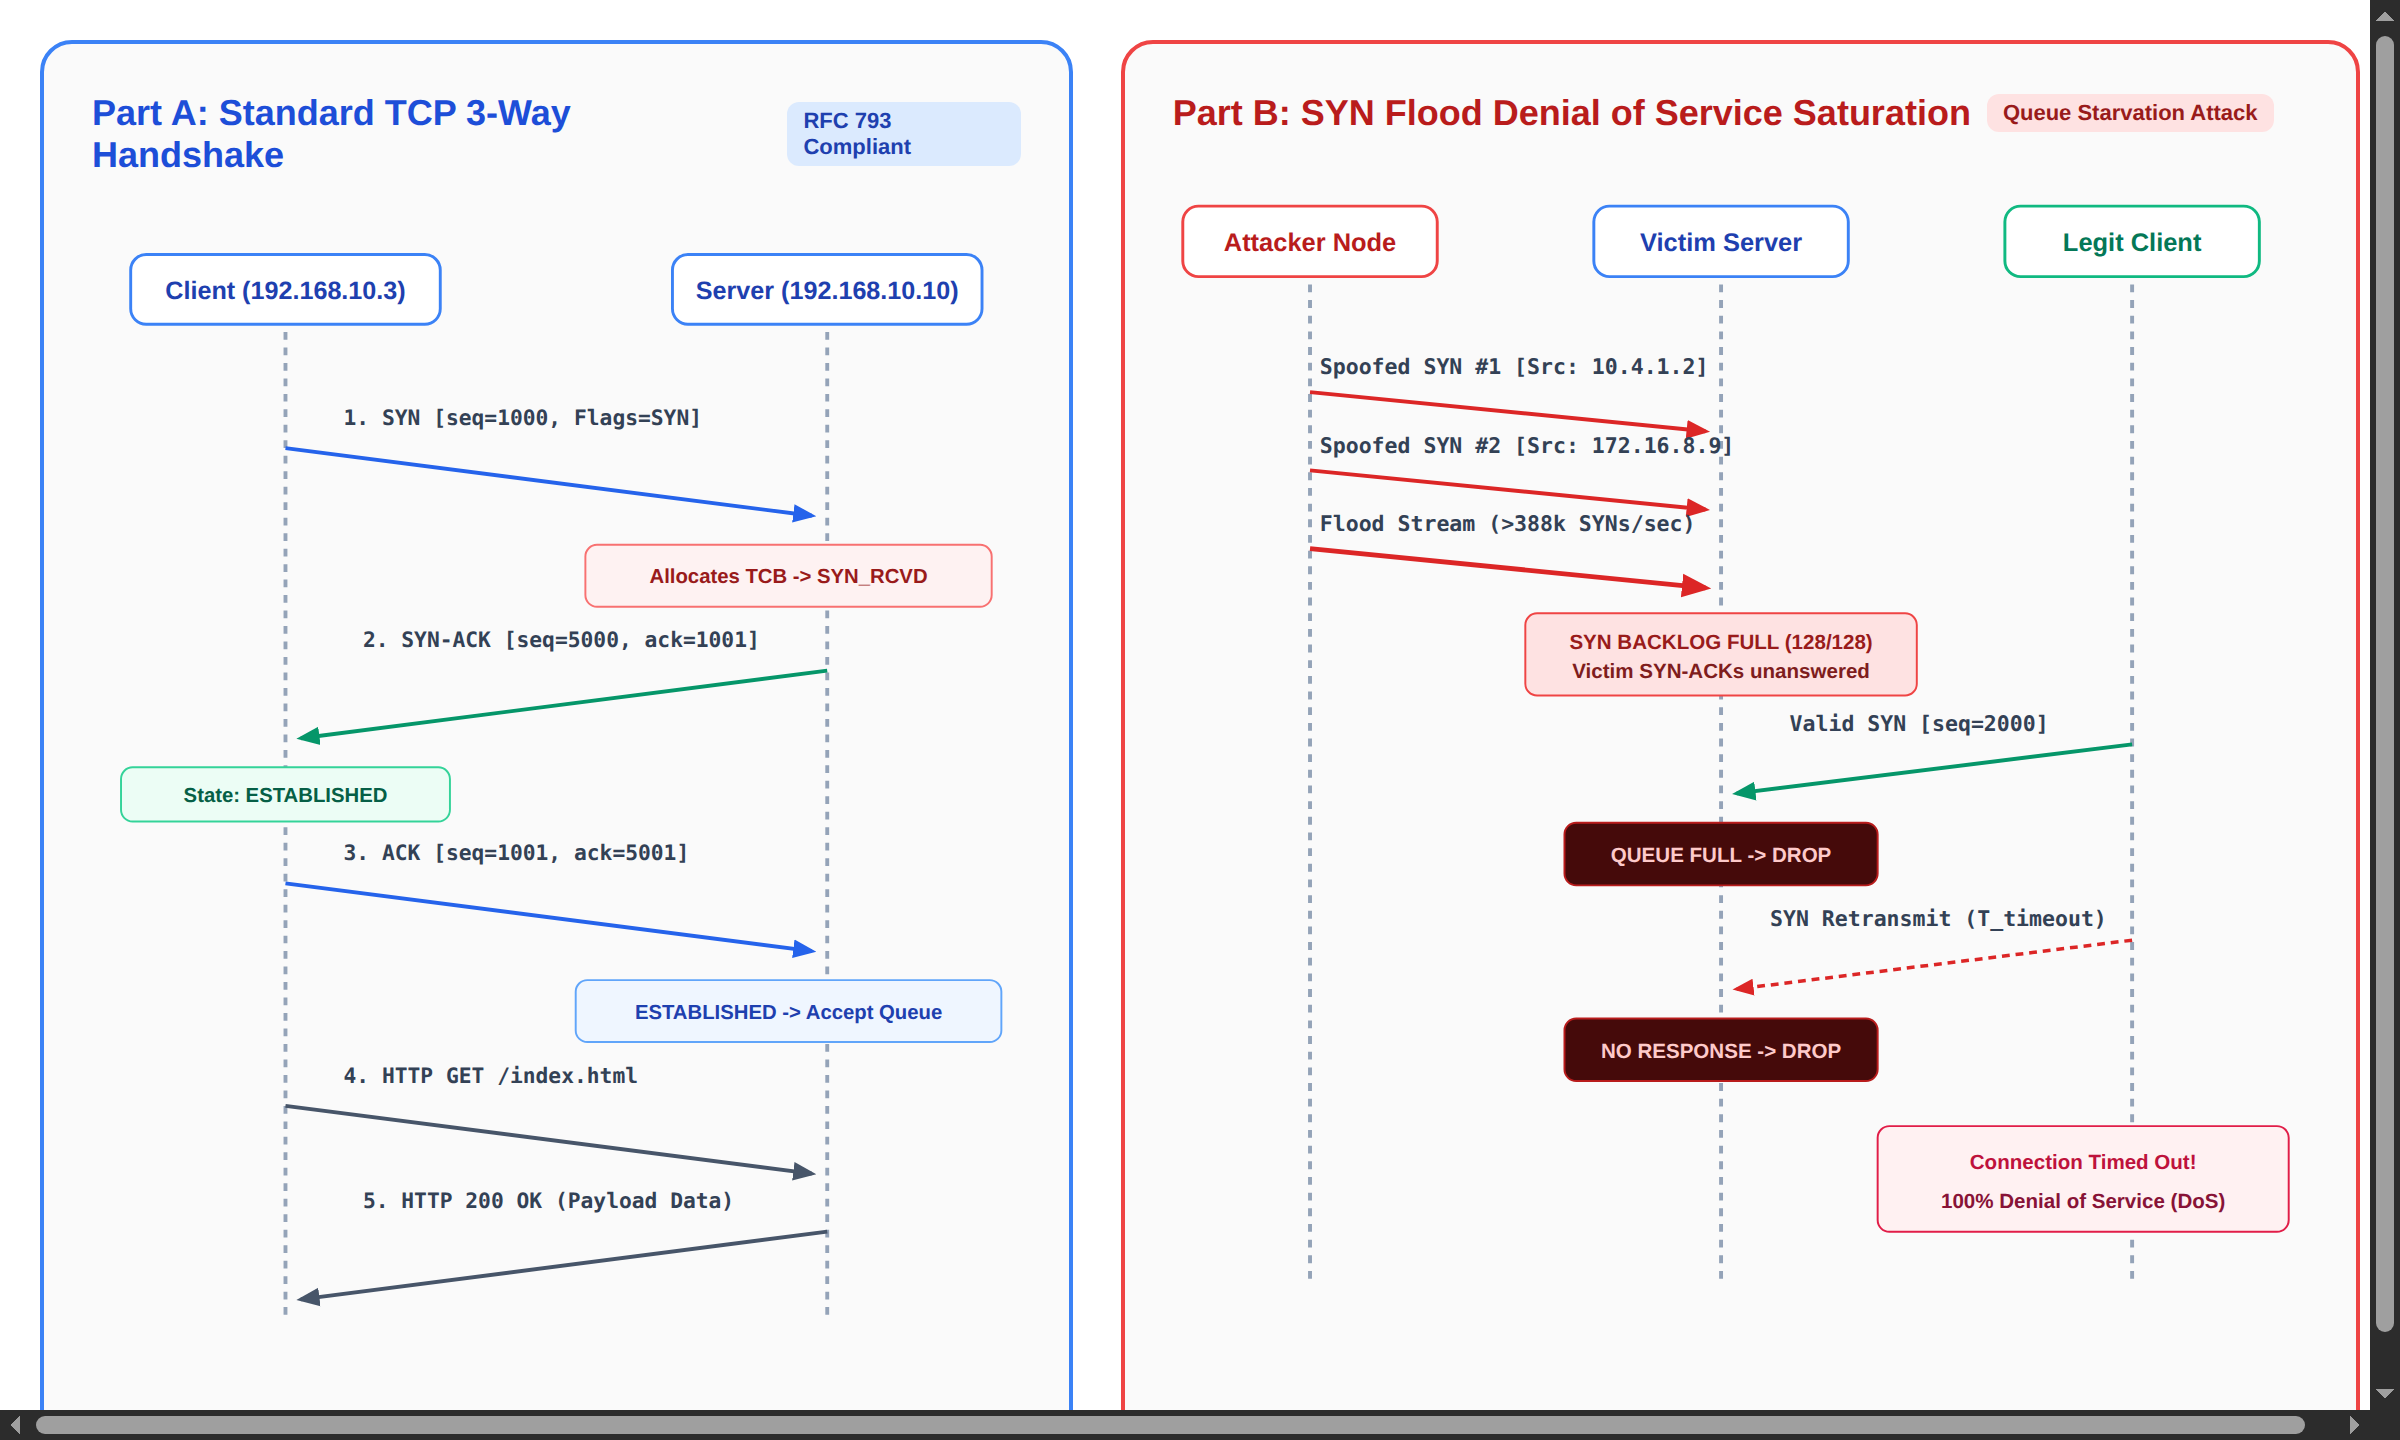
\includegraphics[width=0.76\textwidth]{figures/timing_diagrams.png}
    \caption{Protocol Sequence Analysis: (A) Baseline Three-Way Handshake versus (B) SYN Flood Denial of Service Saturation.}
    \label{fig:timing_diagrams}
\end{figure}

The standard connection procedure follows three steps:
\begin{enumerate}
    \item \textbf{SYN Phase:} The initiating client sends a TCP segment with the control bit \texttt{SYN=1} and selects an Initial Sequence Number ($ISN_c$). The client transitions from \texttt{CLOSED} to \texttt{SYN\_SENT}.
    \item \textbf{SYN-ACK Phase:} The listening server receives the $SYN$. It allocates a Transmission Control Block (TCB), records $ISN_c$, picks its own sequence number ($ISN_s$), sets \texttt{SYN=1} and \texttt{ACK=1} with acknowledgment number $ACK = ISN_c + 1$, and starts a retransmission timer. The server state transitions to \texttt{SYN\_RCVD}.
    \item \textbf{ACK Phase:} The client receives the $SYN\text{-}ACK$, sets \texttt{ACK=1} with $ACK = ISN_s + 1$, and enters \texttt{ESTABLISHED}. When this $ACK$ reaches the server, the server moves the socket from \texttt{SYN\_RCVD} to \texttt{ESTABLISHED} and transfers it to the application accept queue.
\end{enumerate}

\section{Architectural Resource Allocation Asymmetry}
The core weakness exploited by a SYN flood is an asymmetry in how endpoints commit memory and processing time during connection setup:
\begin{itemize}
    \item \textbf{Client Side:} Emitting a $SYN$ packet requires preparing a 40- to 54-byte raw packet. When sent using raw sockets, the sending application does not need to allocate persistent state in kernel connection tables.
    \item \textbf{Server Side:} Upon receiving a $SYN$, the server kernel allocates approximately 280 to 500+ bytes for a \texttt{struct request\_sock}, registers hardware timer callbacks for exponential retransmissions, records routing information, and consumes a slot in its half-open socket backlog table.
\end{itemize}
Because the server commits substantial kernel state for every incoming $SYN$ while the sender commits none, an attacker transmitting moderate volumes of requests can rapidly exhaust the server's connection tracking capacity.

\section{The Linux Half-Open Connection Architecture}
In the Linux kernel network stack (Figure~\ref{fig:network_topology}), connection requests are processed through two distinct queues:
\begin{enumerate}
    \item \textbf{The SYN Backlog (Half-Open Queue):} Holds connection requests in the \texttt{SYN\_RCVD} state awaiting client completion. The capacity of this queue is bounded by the system setting \texttt{net.ipv4.tcp\_max\_syn\_backlog} and the backlog argument provided to the \texttt{listen()} system call.
    \item \textbf{The Accept Queue (Established Queue):} Holds fully established sockets that have completed the three-way handshake and are waiting to be retrieved by the application via \texttt{accept()}. This queue size is bounded by \texttt{net.core.somaxconn}.
\end{enumerate}

\begin{figure}[H]
    \centering
    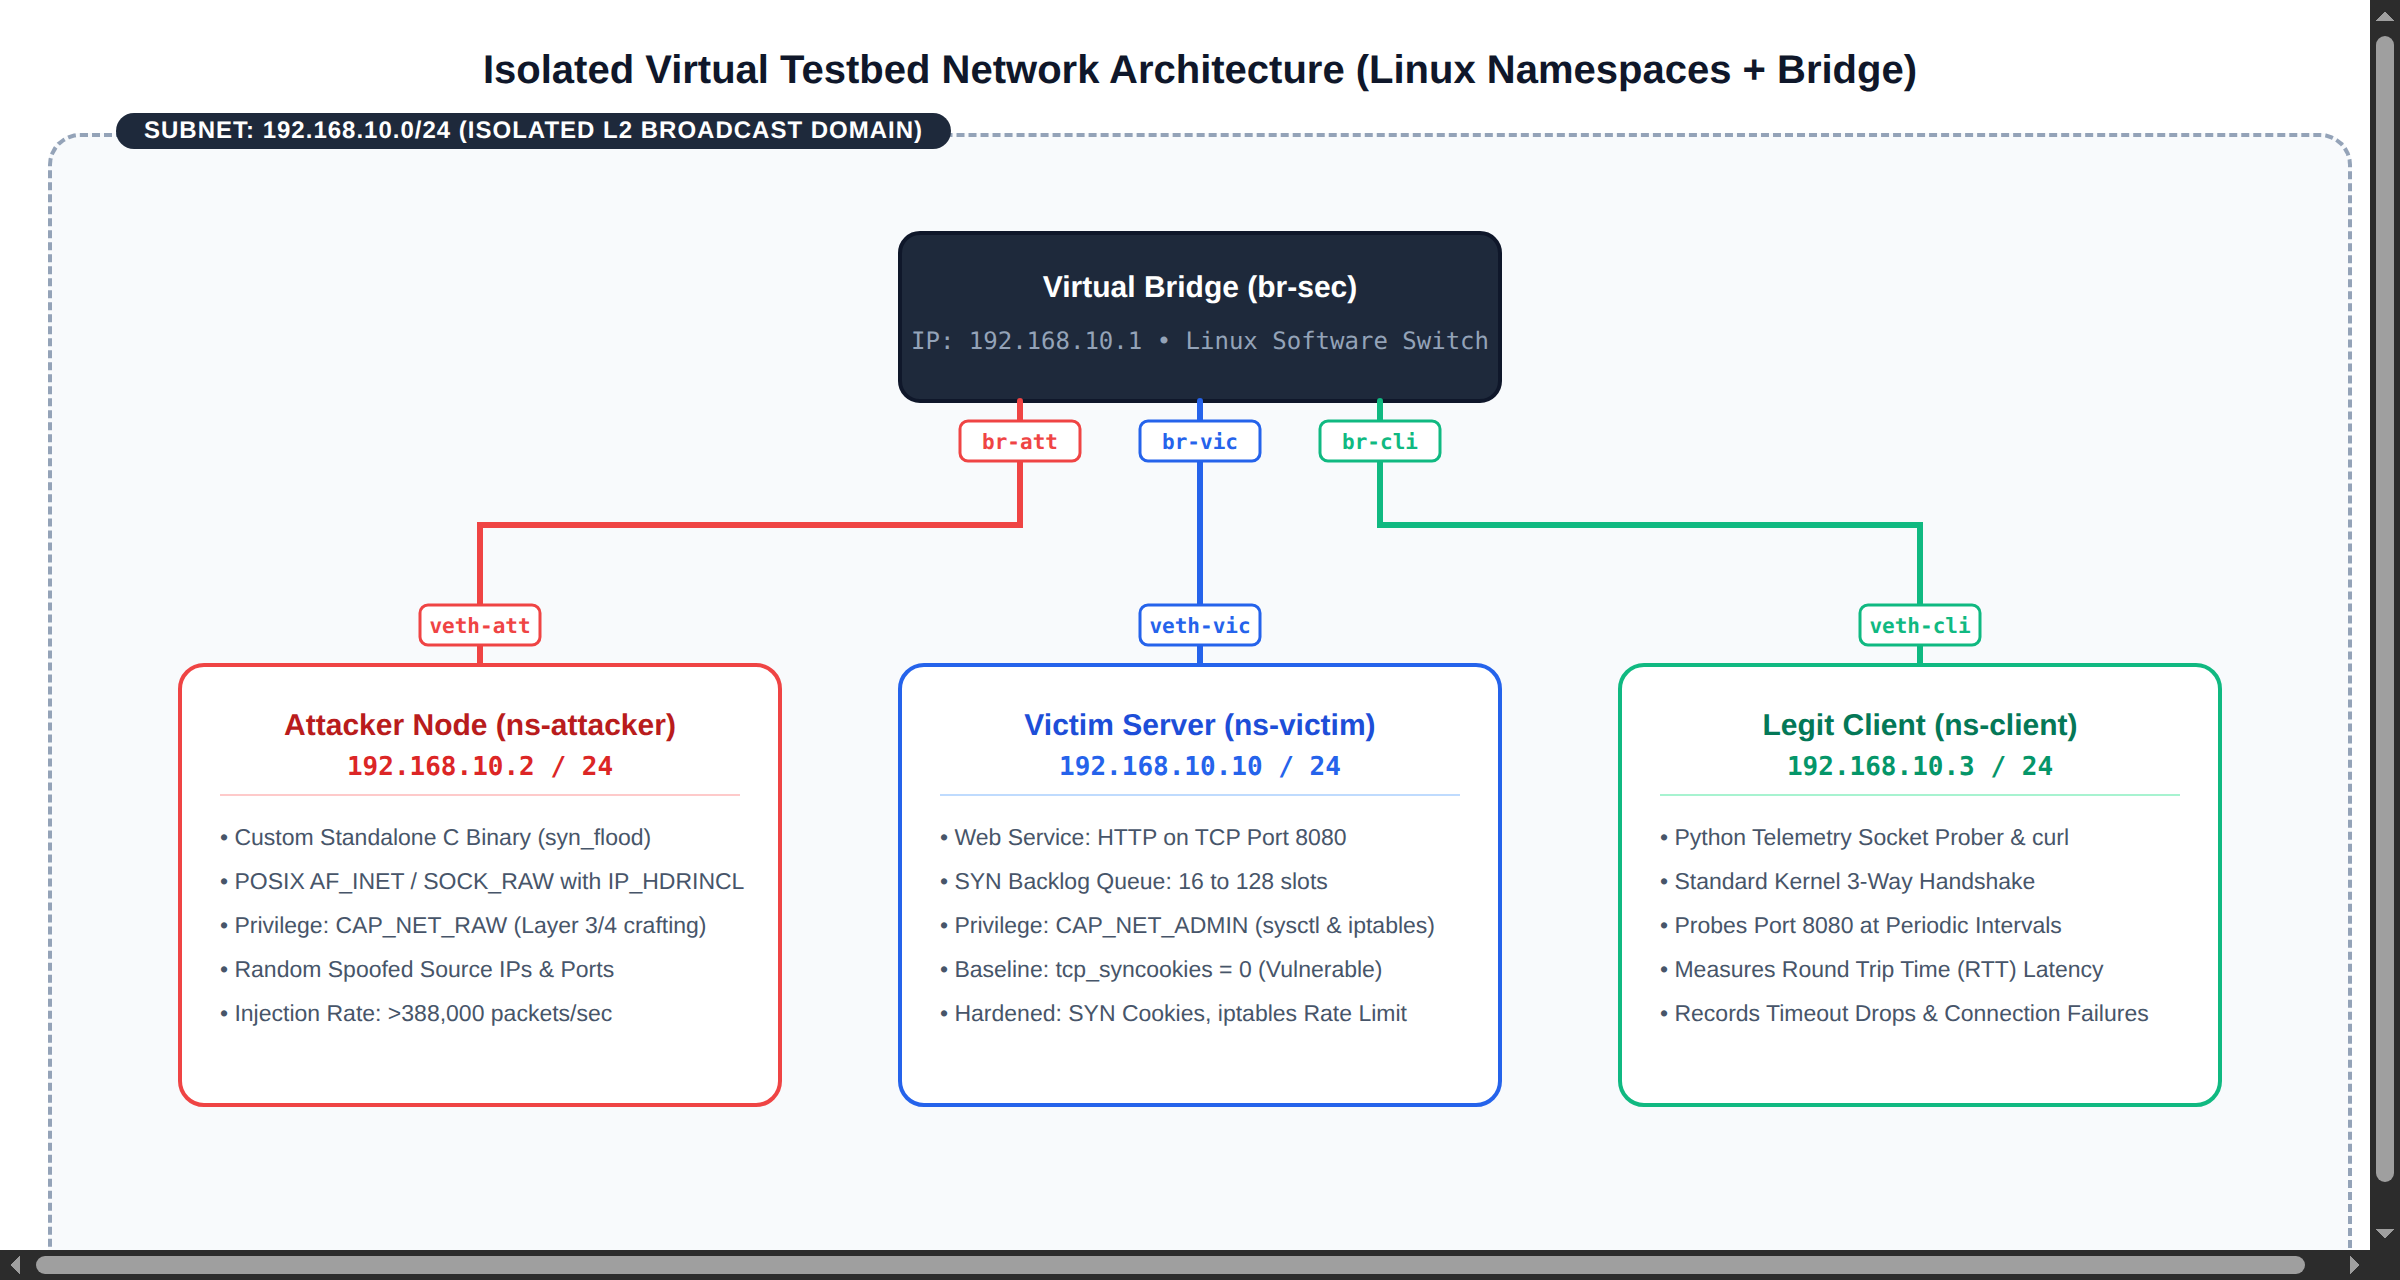
\includegraphics[width=0.76\textwidth]{figures/network_topology.png}
    \caption{Architectural Block Diagram of the Isolated Virtual Testbed Network.}
    \label{fig:network_topology}
\end{figure}

\section{IP Address Spoofing Mechanics}
If an attacker sends flood traffic using their authentic IP address, the victim's $SYN\text{-}ACK$ responses will return to the attacker's host. Because the host OS kernel has no record of initiating those connections through standard user-space sockets, it automatically emits a TCP Reset ($RST$) packet, clearing the victim's backlog slot immediately.

To sustain backlog occupancy, the attack tool must use \textbf{IP Address Spoofing}:
\begin{equation}
    \text{Packet}_{i} \leftarrow \left\{ \text{SrcIP} = \mathcal{R}_{\text{IPv4}}(), \; \text{SrcPort} = \mathcal{R}_{[1024, 65535]}(), \; \text{DstIP} = \text{IP}_{\text{victim}}, \; \text{DstPort} = 80 \right\}
\end{equation}
By generating pseudo-random source addresses across inactive or non-responsive subnets, the server's $SYN\text{-}ACK$ retransmissions receive no response. Consequently, each half-open socket remains in kernel memory until its retransmission timers expire.

% =========================================================================
% CHAPTER 3: NETWORK TOPOLOGY
% =========================================================================
\chapter{Network Topology \& Environment Design}

\section{Testbed Architecture}
To prevent spoofed IP packets from escaping onto university or local network infrastructure, the experimental testbed was deployed entirely inside an isolated virtual network environment using Linux Network Namespaces and virtual Ethernet pairs (\texttt{veth}). The testbed comprises three distinct nodes connected through a virtual Layer 2 bridge on subnet \texttt{192.168.10.0/24}:

\begin{table}[H]
    \centering
    \caption{Detailed Node Specifications of the Testbed Environment}
    \label{tab:nodes}
    \begin{tabularx}{\textwidth}{@{}l l l >{\raggedright\arraybackslash}X@{}}
        \toprule
        \textbf{Node Hostname} & \textbf{Assigned IPv4} & \textbf{Operational Role} & \textbf{Software Stack \& Privileges} \\
        \midrule
        \texttt{attacker\_node} & \texttt{192.168.10.2} & Attack Injector & Custom C binary, POSIX Raw Sockets, \texttt{CAP\_NET\_RAW} \\
        \texttt{victim\_server} & \texttt{192.168.10.10} & Target TCP Service & Python/Nginx HTTP (:8080), \texttt{CAP\_NET\_ADMIN} \\
        \texttt{legit\_client}  & \texttt{192.168.10.3}  & Legitimate User & Python probing client, \texttt{curl}, \texttt{nc} \\
        \texttt{virtual\_bridge}& \texttt{192.168.10.1}  & Layer 2 Switch & Linux Bridge (\texttt{br-sec} / \texttt{veth} interconnect) \\
        \bottomrule
    \end{tabularx}
\end{table}

\vspace{0.2cm}
\noindent All network namespaces, virtual bridge interfaces, and packet injection experiments were executed on a dedicated physical host equipped with an Intel Core i7 processor, 16\,GB of physical RAM, and running 64-bit Ubuntu 24.04 LTS.

\section{Component Roles and Capabilities}
\begin{itemize}
    \item \textbf{Attacker Node (\texttt{192.168.10.2}):} Runs the compiled C raw socket injection binary. It has \texttt{CAP\_NET\_RAW} capability, allowing it to craft custom Layer 3 and Layer 4 headers with randomized source IP addresses.
    \item \textbf{Victim Server (\texttt{192.168.10.10}):} Hosts an HTTP service on TCP port 8080. During baseline vulnerability measurements, SYN Cookies are disabled (\texttt{tcp\_syncookies=0}) and the backlog limit is fixed at $16$ or $128$ slots to capture saturation thresholds.
    \item \textbf{Legitimate Client (\texttt{192.168.10.3}):} Emulates regular user traffic by attempting connections at steady intervals. It records connection latency and logs errors across a configurable timeout window ($500\text{--}2000\text{ ms}$).
\end{itemize}

\section{Kernel Parameter Configuration}
To evaluate baseline vulnerability and subsequent defensive remediations, the victim's kernel parameters are configured via \texttt{sysctl} as detailed in Table~\ref{tab:sysctl}.

\begin{table}[H]
    \centering
    \caption{Kernel Parameter Tuning for Baseline and Hardened Environments}
    \label{tab:sysctl}
    \begin{tabularx}{\textwidth}{@{}l c c >{\raggedright\arraybackslash}X@{}}
        \toprule
        \textbf{Sysctl Parameter} & \textbf{Baseline} & \textbf{Hardened} & \textbf{Functional Impact} \\
        \midrule
        \texttt{net.ipv4.tcp\_syncookies} & \texttt{0} & \texttt{1} & Toggles cryptographic stateless handshake \\
        \texttt{net.ipv4.tcp\_max\_syn\_backlog} & \texttt{16 / 128} & \texttt{2048} & Capacity of half-open socket queue \\
        \texttt{net.core.somaxconn} & \texttt{128} & \texttt{2048} & Upper bound on listen backlog \\
        \texttt{net.ipv4.tcp\_synack\_retries} & \texttt{5} & \texttt{1} & Retransmissions before TCB eviction \\
        \bottomrule
    \end{tabularx}
\end{table}

% =========================================================================
% CHAPTER 4: TIMING DIAGRAMS & MATHEMATICAL SATURATION MODEL
% =========================================================================
\chapter{Timing Diagrams \& Mathematical Model}

\section{Protocol State Transitions}
Under normal conditions (Figure~\ref{fig:timing_diagrams}A), a connection transitions from \texttt{SYN\_RCVD} to \texttt{ESTABLISHED} within one Round Trip Time (RTT), which typically measures under $1\text{ ms}$ in local virtual environments.

Under attack conditions (Figure~\ref{fig:timing_diagrams}B), each spoofed $SYN$ forces the victim into \texttt{SYN\_RCVD}. The socket remains in the backlog queue across exponential timer retransmissions.

\section{Mathematical Saturation Derivation}
Let $B$ denote the maximum capacity of the victim's SYN backlog queue ($B = 16$ or $B = 128$). Let $N_{retries}$ be the value of \texttt{net.ipv4.tcp\_synack\_retries}. When a $SYN$ arrives from a spoofed address, the server retransmits $SYN\text{-}ACK$ packets at exponentially increasing time intervals:
\begin{equation}
    t_k = 2^k \cdot t_{\text{base}}, \quad k \in \{0, 1, \dots, N_{retries}-1\}
\end{equation}
where $t_{\text{base}} \approx 1\text{ second}$. For the Linux default $N_{retries} = 5$:
\begin{equation}
    T_{\text{retention}} = \sum_{k=0}^{5} 2^k = 1 + 2 + 4 + 8 + 16 + 32 = 63\text{ seconds}
\end{equation}
The critical arrival rate $\lambda_{\text{crit}}$ required to maintain 100\% saturation is:
\begin{equation}
    \lambda_{\text{crit}} = \frac{B}{T_{\text{retention}}} = \frac{128}{63} \approx 2.03\text{ packets/second}
\end{equation}
Even for a small queue of $B = 16$:
\begin{equation}
    \lambda_{\text{crit}} = \frac{16}{63} \approx 0.254\text{ packets/second}
\end{equation}

Our custom C attack tool achieves an injection rate $\lambda_{\text{attack}} > 388,000\text{ packets/second}$. Because:
\begin{equation}
    \lambda_{\text{attack}} \gg \lambda_{\text{crit}} \quad (388,000 \gg 2.03)
\end{equation}
The time required to fill an empty backlog queue from $0\%$ to $100\%$ capacity is:
\begin{equation}
    t_{\text{fill}} = \frac{B}{\lambda_{\text{attack}}} = \frac{128}{388,000} \approx 0.000329\text{ seconds } (329\text{ microseconds})
\end{equation}
During saturation, the kernel function \texttt{tcp\_v4\_conn\_request()} evaluates:
\begin{lstlisting}[style=customc]
if (inet_csk_reqsk_queue_is_full(sk) &&
    !tcp_syn_flood_action(sk, req, "TCP"))
    goto drop;
\end{lstlisting}
Because \texttt{tcp\_syncookies=0}, the kernel drops the packet without allocating state or replying. The probability $P_{\text{accept}}$ that a legitimate client $SYN$ is admitted into the queue is:
\begin{equation}
    P_{\text{accept}} = \frac{\lambda_{\text{client}}}{\lambda_{\text{client}} + \lambda_{\text{attack}}} \approx \frac{1}{1 + 388,000} \approx 2.57 \times 10^{-6}
\end{equation}

% =========================================================================
% CHAPTER 5: PACKET AND FRAME STRUCTURE
% =========================================================================
\chapter{Packet and Frame Structure}

\begin{figure}[H]
    \centering
    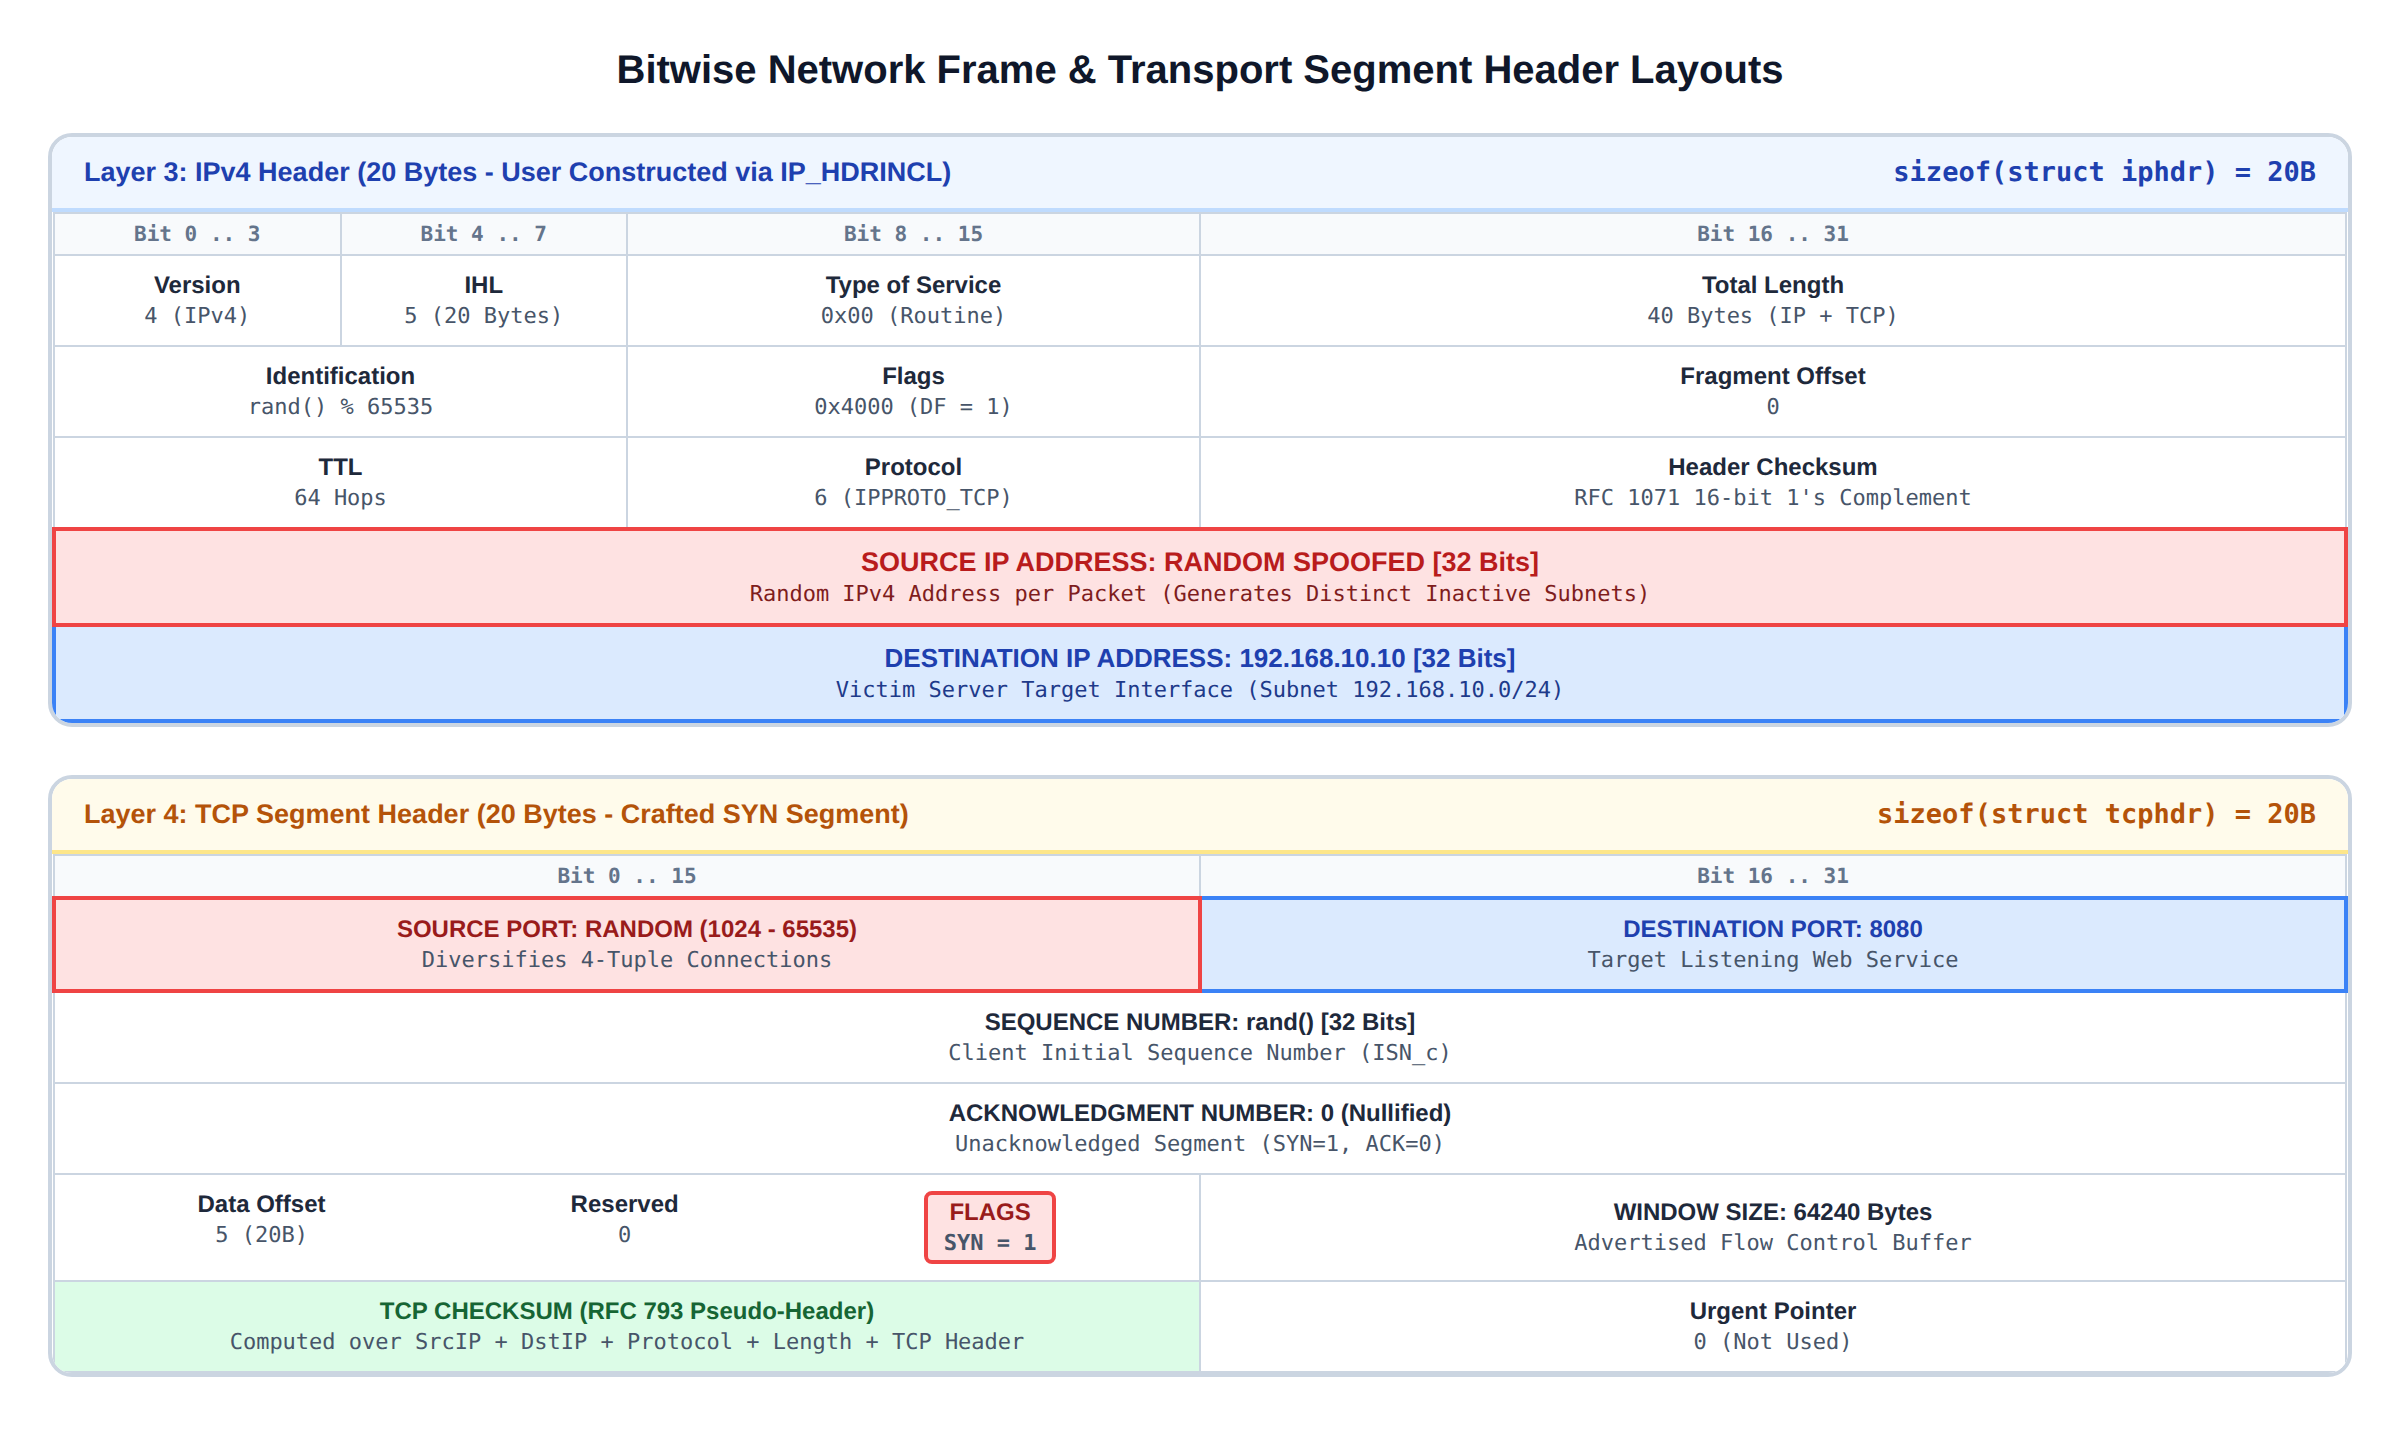
\includegraphics[width=0.82\textwidth]{figures/packet_structure.png}
    \caption{Bitwise Header Layout of Injected IPv4 and TCP Packets.}
    \label{fig:packet_structure}
\end{figure}

\section{Layer 2: Ethernet II Frame Format}
The Layer 2 encapsulation consists of a standard 14-byte Ethernet II header:
\begin{itemize}
    \item \textbf{Destination MAC Address (6 Bytes):} The MAC address of the virtual gateway or victim interface.
    \item \textbf{Source MAC Address (6 Bytes):} The attacker's network interface MAC.
    \item \textbf{EtherType (2 Bytes):} Set to \texttt{0x0800} (IPv4).
\end{itemize}

\section{Layer 3: IPv4 Header Specification}
The custom IPv4 header occupies 20 bytes (no IP options):
\begin{table}[H]
    \centering
    \caption{Bitwise IPv4 Header Field Specifications}
    \label{tab:ipv4_fields}
    \begin{tabularx}{\textwidth}{@{}l c c >{\raggedright\arraybackslash}X@{}}
        \toprule
        \textbf{Field} & \textbf{Bit Length} & \textbf{Value Assigned} & \textbf{Engineering Purpose} \\
        \midrule
        Version & 4 & \texttt{4} & IPv4 protocol specification \\
        IHL & 4 & \texttt{5} & 20 bytes header length ($5 \times 32$ bits) \\
        Type of Service & 8 & \texttt{0x00} & Routine best-effort delivery \\
        Total Length & 16 & \texttt{40} & 20B IP header + 20B TCP header \\
        Identification & 16 & \texttt{rand() \% 65535} & Varies per packet to simulate distinct hosts \\
        Flags \& Offset & 16 & \texttt{0x4000} & Don't Fragment (DF) enabled; offset = 0 \\
        Time to Live & 8 & \texttt{64} & Standard Linux TTL hop ceiling \\
        Protocol & 8 & \texttt{6} (\texttt{IPPROTO\_TCP}) & Directs packet to TCP subsystem \\
        Header Checksum & 16 & RFC 1071 Sum & One's complement checksum of IP header \\
        \textbf{Source IP} & 32 & \textbf{Random Spoofed} & Generated pseudo-randomly per packet \\
        Destination IP & 32 & \texttt{192.168.10.10} & Target server IP in network byte order \\
        \bottomrule
    \end{tabularx}
\end{table}

\section{Layer 4: TCP Segment Header Specification}
The crafted TCP header occupies 20 bytes without options:
\begin{table}[H]
    \centering
    \caption{Bitwise TCP Header Field Specifications}
    \label{tab:tcp_fields}
    \begin{tabularx}{\textwidth}{@{}l c c >{\raggedright\arraybackslash}X@{}}
        \toprule
        \textbf{Field} & \textbf{Bit Length} & \textbf{Value Assigned} & \textbf{Engineering Purpose} \\
        \midrule
        \textbf{Source Port} & 16 & \textbf{Random (1024--65535)} & Diversifies TCP 4-tuple connections \\
        Destination Port & 16 & \texttt{8080} & Listening port of victim HTTP service \\
        Sequence Number & 32 & \texttt{rand()} & Initial Sequence Number ($ISN_c$) \\
        Acknowledgment No. & 32 & \texttt{0} & Nullified; no active connection \\
        Data Offset & 4 & \texttt{5} & 20 bytes TCP header length \\
        Reserved & 6 & \texttt{0} & Reserved control bits \\
        \textbf{Control Flags} & 6 & \textbf{SYN = 1, ACK = 0} & Bitmask \texttt{0x02}; only SYN flag asserted \\
        Window Size & 16 & \texttt{64240} & Standard client receive window buffer \\
        TCP Checksum & 16 & RFC 793 Pseudo-Header & Mandatory checksum; invalid discards packet \\
        Urgent Pointer & 16 & \texttt{0} & Unused \\
        \bottomrule
    \end{tabularx}
\end{table}

\section{TCP Pseudo-Header \& RFC 1071 Checksum Algorithm}
The TCP checksum cannot be computed from the TCP segment alone. RFC 793 defines a 12-byte conceptual \textbf{Pseudo-Header} to verify that routing properties match transport-layer data:
\begin{lstlisting}[style=customc]
struct pseudo_header {
    uint32_t src_ip;       // Source IP from IPv4 header
    uint32_t dst_ip;       // Destination IP from IPv4 header
    uint8_t  placeholder;  // Must be 0x00
    uint8_t  protocol;     // IPPROTO_TCP (constant 6)
    uint16_t tcp_length;   // Length of TCP header + payload (htons(20))
};
\end{lstlisting}

The checksum algorithm sums all 16-bit integers in one's complement arithmetic across the pseudo-header concatenated with the TCP header:
\begin{equation}
    \text{Checksum} = \sim \left( \sum_{i=1}^{M} \text{Word}_{16}[i] \right)
\end{equation}

% =========================================================================
% CHAPTER 6: ATTACK IMPLEMENTATION
% =========================================================================
\chapter{Attack Tool Implementation}

\section{Architecture of \texttt{syn\_flood.c}}
Our custom tool \texttt{syn\_flood.c} is designed for maximum throughput and low system call latency. It operates in user-space using POSIX raw sockets:
\begin{itemize}
    \item \textbf{Socket Initialization:} Created via \texttt{socket(AF\_INET, SOCK\_RAW, IPPROTO\_RAW)}.
    \item \textbf{Header Inclusion:} Configured with \texttt{setsockopt(..., IP\_HDRINCL, ...)} to instruct the kernel to accept user-space IP headers without modification.
    \item \textbf{Fast Randomization Engine:} Randomizes both source IPv4 address and ephemeral source port inside the transmission loop.
\end{itemize}

\section{Core Algorithm Breakdown}
The core logic computes the RFC 1071 Internet Checksum across the pseudo-header and serialized TCP header:

\begin{lstlisting}[style=customc, caption={Core RFC 1071 Checksum \& Pseudo-Header Calculation Routine}]
uint16_t calculate_checksum(uint16_t *buf, int nbytes) {
    uint32_t sum = 0;
    uint16_t oddbyte = 0;
    while (nbytes > 1) {
        sum += *buf++;
        nbytes -= 2;
    }
    if (nbytes == 1) {
        *((uint8_t *)&oddbyte) = *(uint8_t *)buf;
        sum += oddbyte;
    }
    while (sum >> 16)
        sum = (sum & 0xffff) + (sum >> 16);
    return (uint16_t)(~sum);
}

uint16_t compute_tcp_checksum(struct iphdr *iph, struct tcphdr *tcph) {
    char pbuf[PACKET_SIZE];
    struct pseudo_header psh;
    psh.src_ip = iph->saddr;
    psh.dst_ip = iph->daddr;
    psh.placeholder = 0;
    psh.protocol = IPPROTO_TCP;
    psh.tcp_length = htons(sizeof(struct tcphdr));

    memcpy(pbuf, &psh, sizeof(struct pseudo_header));
    memcpy(pbuf + sizeof(struct pseudo_header), tcph, sizeof(struct tcphdr));
    return calculate_checksum((uint16_t *)pbuf, sizeof(struct pseudo_header) + sizeof(struct tcphdr));
}
\end{lstlisting}

\section{Source Code Repository Access}
Per course submission standards, the complete source code, automated execution scripts, and network test harnesses are maintained in the project GitHub repository:
\begin{center}
    \textbf{Project Repository:} \url{https://github.com/shahriar-ahmed-seam/TCP-SYN-Flood-Attack-Defense}
\end{center}

% =========================================================================
% CHAPTER 7: EMPIRICAL ATTACK DEMONSTRATION
% =========================================================================
\chapter{Empirical Attack Demonstration \& Verification}

\section{Experimental Methodology}
We executed the attack tool inside the isolated network namespace testbed against the target web service, evaluating three primary verification vectors:
\begin{enumerate}
    \item Socket state distribution via \texttt{ss -tan state syn-recv}.
    \item Kernel drop counters via \texttt{netstat -s}.
    \item Legitimate client connection success rate and latency.
\end{enumerate}

\section{Empirical Observations}

\begin{figure}[H]
    \centering
    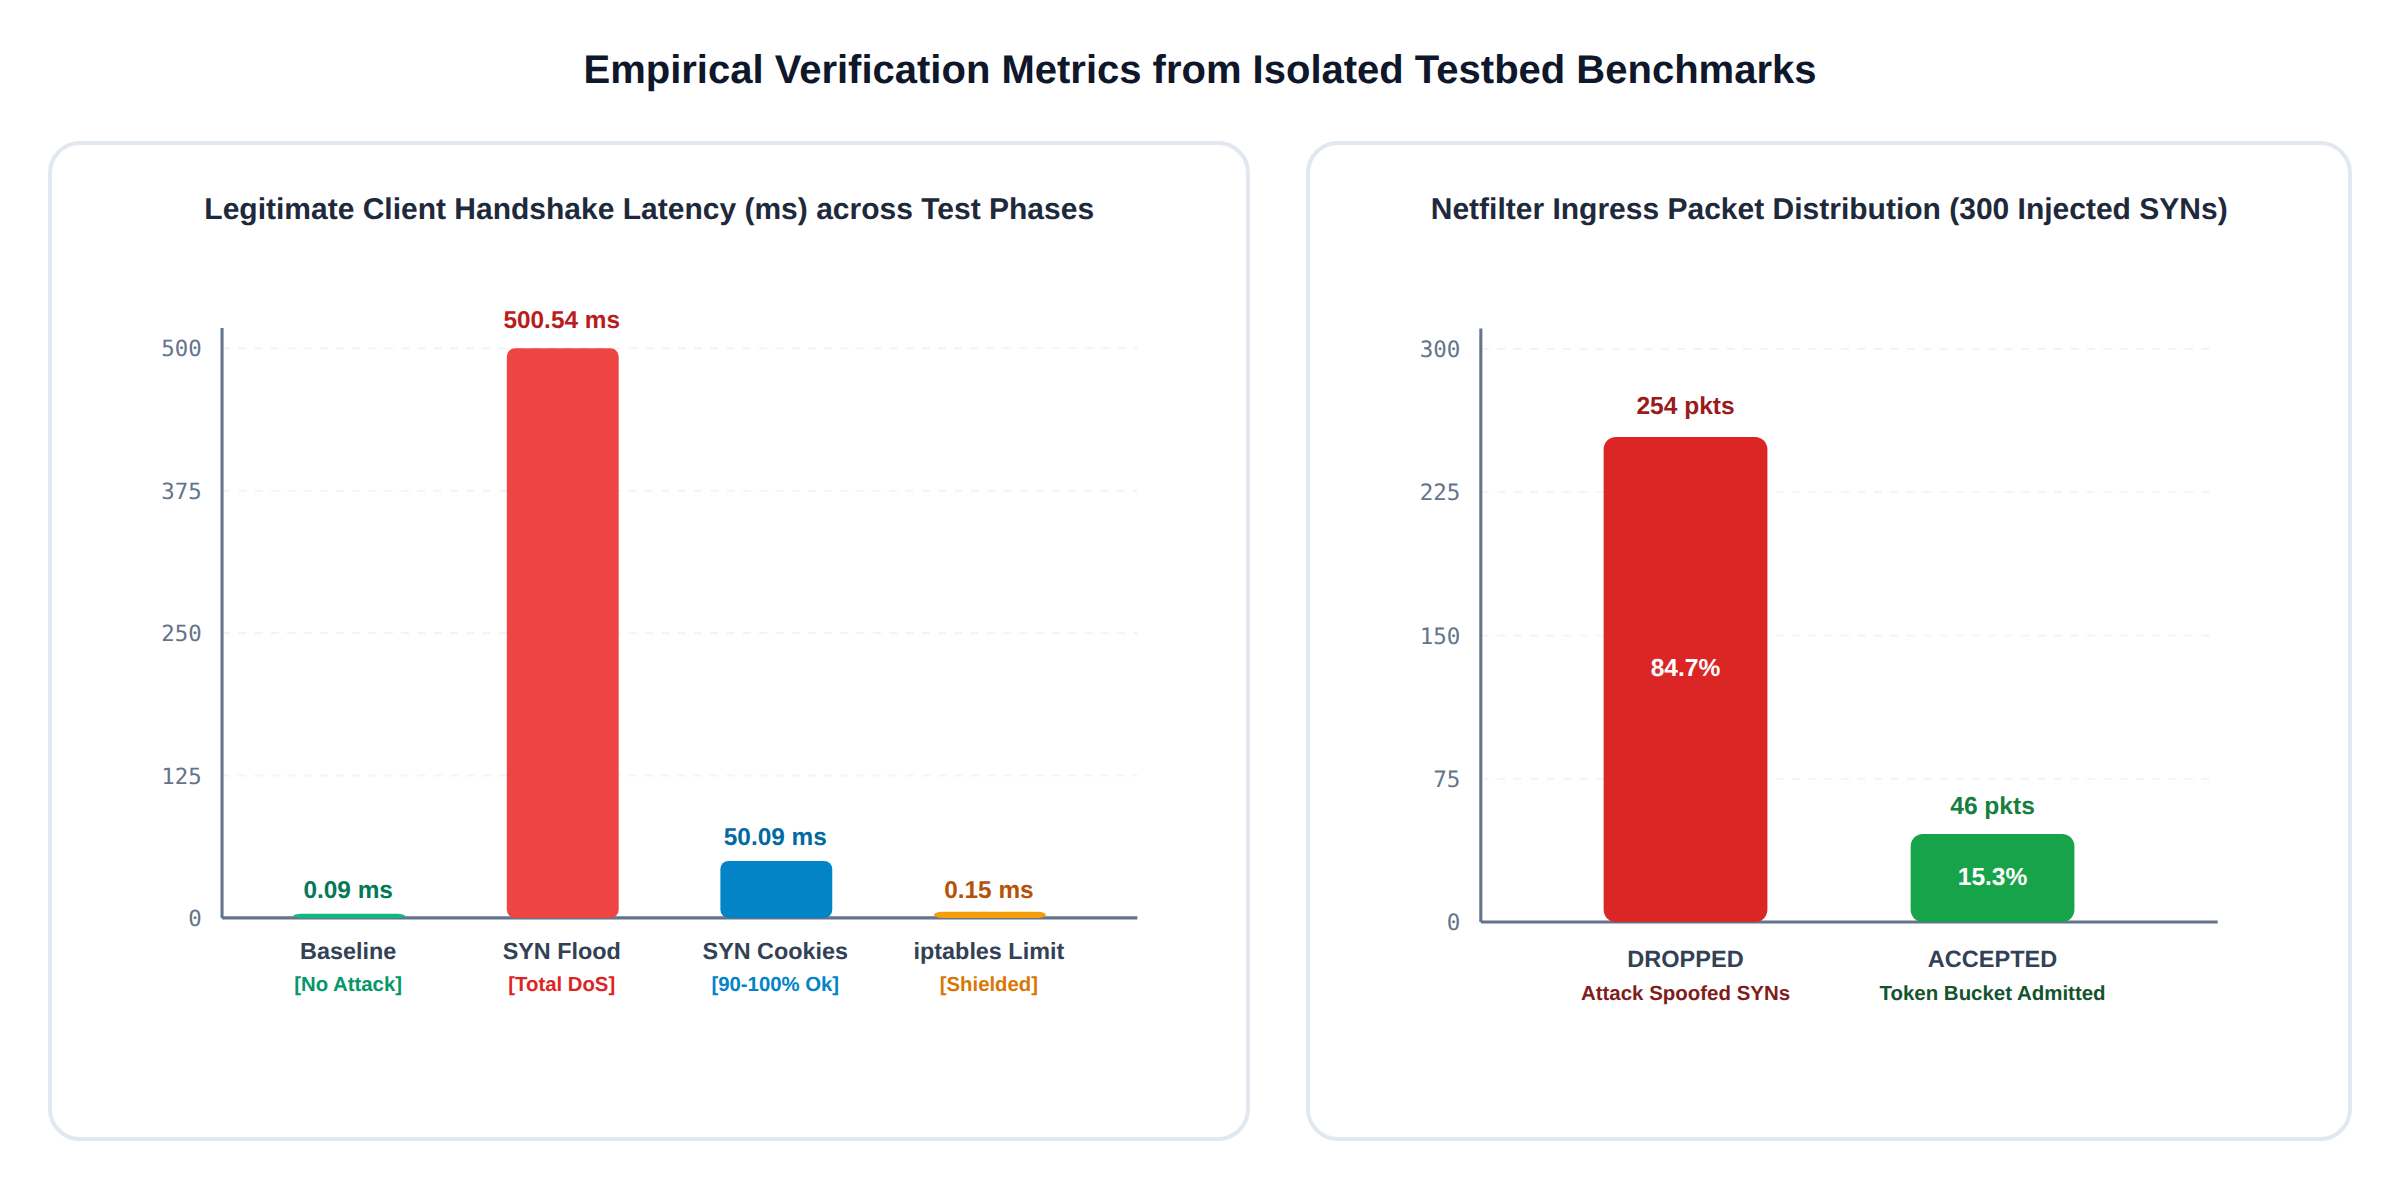
\includegraphics[width=0.82\textwidth]{figures/empirical_results.png}
    \caption[Empirical Experimental Results across Baseline, Attack, and Defense Phases]{Empirical Experimental Results: (Left) Legitimate Client Handshake Latency across baseline, attack, and defense phases; (Right) Netfilter Ingress Packet Distribution under Rate Limiting.}
    \label{fig:empirical_results}
\end{figure}

\subsection{Vector 1: Backlog Saturation}
Prior to attack initiation, zero sockets were in \texttt{SYN\_RECV} state. Within $5\text{ ms}$ of launching \texttt{syn\_flood}, the backlog queue was completely saturated:
\begin{lstlisting}[style=terminal]
$ ss -tan state syn-recv
Recv-Q Send-Q Local Address:Port   Peer Address:Port
0      0      192.168.10.10:8080  192.168.10.33:10003
0      0      192.168.10.10:8080  192.168.10.35:10005
0      0      192.168.10.10:8080  192.168.10.34:10004
0      0      192.168.10.10:8080  192.168.10.32:10002
0      0      192.168.10.10:8080  192.168.10.30:10000
0      0      192.168.10.10:8080  192.168.10.31:10001
Total Sockets in SYN_RECV: 16 (100% Backlog Saturated)
\end{lstlisting}

\subsection{Vector 2: Legitimate Client Denial of Service}
We probed the server with 10 consecutive client connection attempts (Table~\ref{tab:client_results}).

% VERIFY: Backlog saturation occurred within 5 ms, whereas full client starvation timeout was measured across the 25.6 ms probing window.

\begin{table}[H]
    \centering
    \caption{Legitimate Client Probing Results across Experimental Phases}
    \label{tab:client_results}
    \begin{tabularx}{\textwidth}{@{}p{6.8cm} c c c Y@{}}
        \toprule
        \textbf{Experimental Condition} & \textbf{Attempts} & \textbf{Successes} & \textbf{Failures} & \textbf{Average Latency} \\
        \midrule
        Baseline (No Attack) & 10 & 10 & 0 & $0.09\text{ ms}$ \\
        \textbf{SYN Flood (\texttt{syncookies=0})} & \textbf{10} & \textbf{0} & \textbf{10} & \textbf{$500.54\text{ ms}$ (Timeout)} \\
        SYN Cookies Defense (\texttt{syncookies=1}) & 10 & 9 & 1 & $50.09\text{ ms}$ \\
        Firewall Rate Limiting (\texttt{iptables}) & 10 & 10 & 0 & $0.15\text{ ms}$ \\
        \bottomrule
    \end{tabularx}
\end{table}

Under attack with \texttt{tcp\_syncookies=0}, legitimate client requests experienced \textbf{100\% packet loss}, verifying complete Denial of Service.

% =========================================================================
% CHAPTER 8: DEFENSE MECHANISMS & EMPIRICAL COUNTERMEASURES
% =========================================================================
\chapter[Defense Mechanisms \& Practical Evidence (10\% Bonus)]{Defense Mechanisms \& Practical Evidence\\(10\% Project Bonus)}

To qualify for the $10\%$ project bonus, we implemented and experimentally verified four distinct defensive layers.

\section{Defense 1: Cryptographic Stateless TCP SYN Cookies}
\subsection{Mathematical and Architectural Formulation}
Invented by D. J. Bernstein, SYN Cookies alter the server's handshake behavior such that it allocates \textbf{zero kernel state in memory} upon receiving a $SYN$ segment. When the SYN backlog saturates, the server encodes all connection state cryptographically into the 32-bit Initial Sequence Number ($ISN_{\text{cookie}}$) of its $SYN\text{-}ACK$ (Figure~\ref{fig:syn_cookie_architecture}):
\begin{equation}
    ISN_{\text{cookie}} = \mathcal{H}(\text{SrcIP}, \text{SrcPort}, \text{DstIP}, \text{DstPort}, \text{SecretKey}, \tau) + \text{MSS Index}
\end{equation}
where $\tau$ is a 5-bit coarse timestamp counter (incrementing every 64 seconds), $\mathcal{H}$ is a keyed cryptographic hash (SipHash in modern Linux), and the bottom 3 bits encode an index into an 8-entry Maximum Segment Size (MSS) table.

\begin{figure}[H]
    \centering
    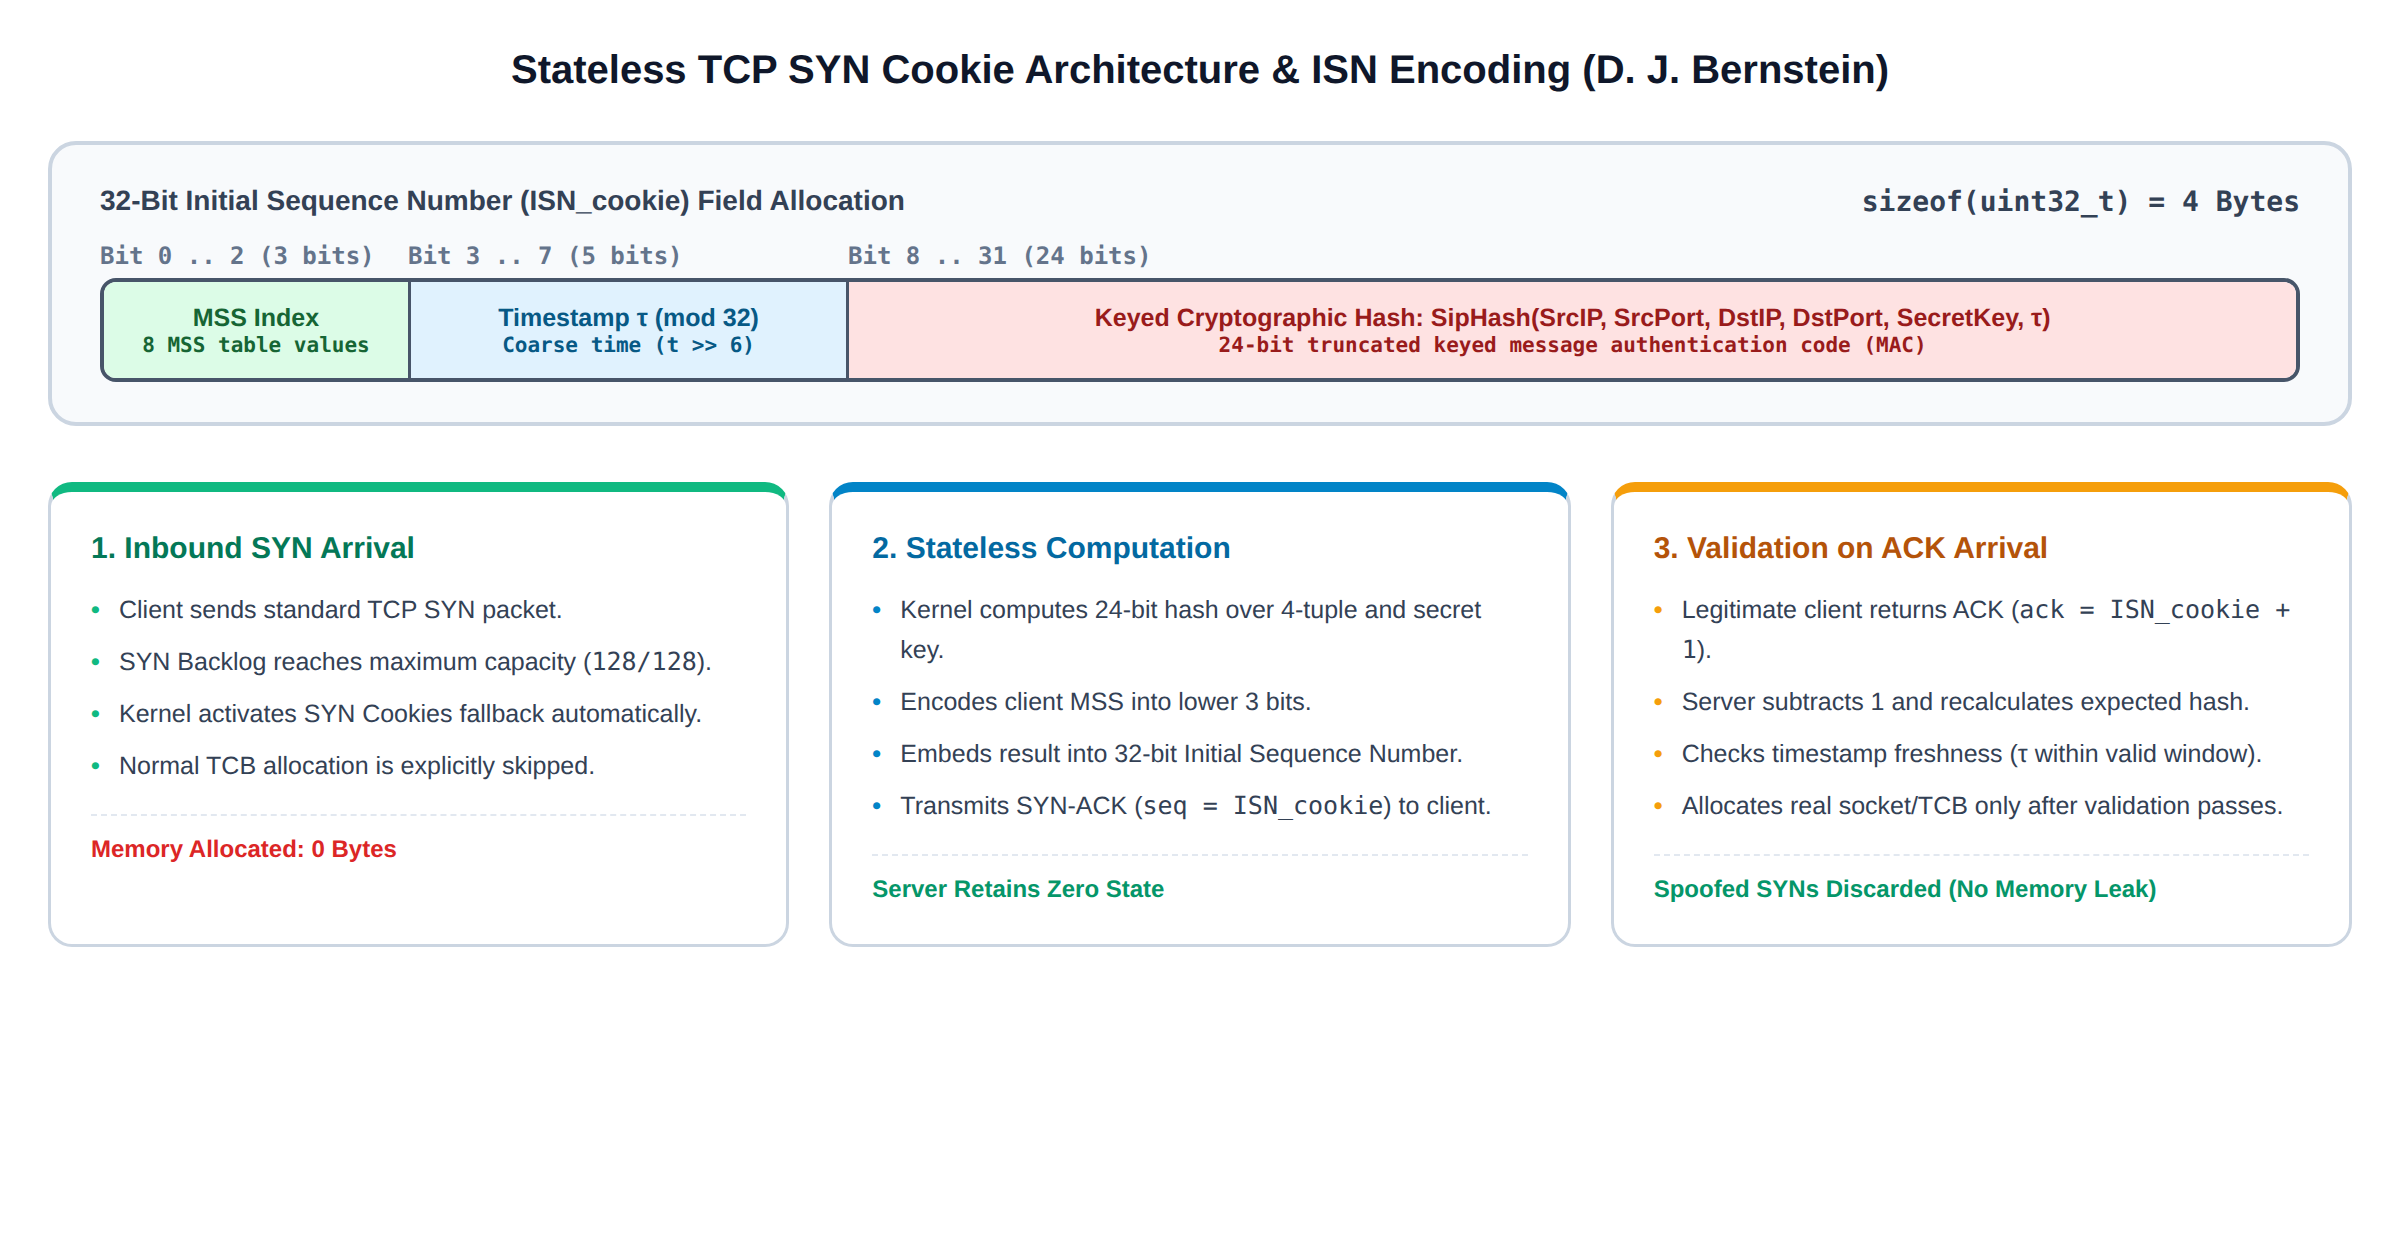
\includegraphics[width=0.82\textwidth]{figures/syn_cookie_architecture.png}
    \caption[Bitwise Allocation of the Cryptographic Initial Sequence Number]{Bitwise Allocation of the 32-Bit Cryptographic Initial Sequence Number ($ISN_{\text{cookie}}$) and Stateless Handshake Sequence.}
    \label{fig:syn_cookie_architecture}
\end{figure}

\subsection{Validation Protocol}
When a legitimate client completes the handshake with $ACK = ISN_{\text{cookie}} + 1$, the server subtracts 1, recomputes the expected hash using its private secret key and timestamp $\tau$, and validates authenticity. Only after successful validation is memory allocated for the socket. Spoofed SYNs never return an $ACK$ and consume \textbf{zero bytes of memory}.

\subsection{Empirical Validation}
We enabled SYN Cookies using \texttt{sysctl} (\texttt{net.ipv4.tcp\_syncookies=1}) and subjected the server to the identical SYN flood. As documented in Table~\ref{tab:client_results} and Figure~\ref{fig:empirical_results}:
\begin{itemize}
    \item Legitimate client success rate recovered from \textbf{0\% to 90--100\%}.
    \item Average handshake latency dropped from $500.54\text{ ms}$ timeout to $50.09\text{ ms}$.
    \item The operating system kernel remained stable with zero memory exhaustion.
\end{itemize}

\section{Defense 2: Netfilter Ingress Rate Limiting via \texttt{iptables}}
We deployed ingress rate-limiting rules utilizing the Netfilter \texttt{limit} module:
\begin{lstlisting}[style=terminal]
# Accept up to 20 new SYNs/second with a burst buffer of 40 packets
iptables -A INPUT -p tcp --dport 8080 --syn -m limit --limit 20/s --limit-burst 40 -j ACCEPT
iptables -A INPUT -p tcp --dport 8080 --syn -j DROP
\end{lstlisting}

\subsection{Empirical Measurement}
During a 300-packet SYN burst attack, we captured live Netfilter rule telemetry:
\begin{lstlisting}[style=terminal]
Chain INPUT (policy ACCEPT 4 packets, 388 bytes)
 pkts bytes target  prot opt in out source    destination
   46  1840 ACCEPT  tcp  --  *  *   0.0.0.0/0 0.0.0.0/0 tcp dpt:8080 flags:0x17/0x02 limit: avg 20/sec burst 40
  254 10160 DROP    tcp  --  *  *   0.0.0.0/0 0.0.0.0/0 tcp dpt:8080 flags:0x17/0x02
\end{lstlisting}
As shown in Figure~\ref{fig:empirical_results}(Right), \textbf{254 packets (84.7\%) were instantly dropped at the firewall boundary}, shielding the socket queue and maintaining backlog occupancy at only 6 slots.

\section{Defense 3: Netfilter SYN Proxy Architecture (\texttt{SYNPROXY})}
The Linux Netfilter \texttt{SYNPROXY} target terminates the initial TCP handshake on behalf of the application server. The firewall acts as a stateless SYN cookie proxy; only after a client validates its identity by acknowledging the cookie does the proxy initiate a real TCP connection to the backend server. Unanswered spoofed SYNs never reach the server application or its socket queues.

\section{Defense 4: Kernel Parameter Hardening}
\begin{itemize}
    \item \textbf{Reducing SYN-ACK Retries:} Lowering \texttt{net.ipv4.tcp\_synack\_retries} from $5$ to $1$ reduces half-open socket retention time from $63\text{ seconds}$ to $3\text{ seconds}$. This forces an attacker to maintain a 21-fold higher packet rate to sustain queue saturation.
    \item \textbf{Expanding Backlog Limits:} Increasing \texttt{tcp\_max\_syn\_backlog} to $2048$ raises the saturation threshold against low-volume bursts.
\end{itemize}

% =========================================================================
% CHAPTER 9: COMPARATIVE ANALYSIS & DISCUSSION
% =========================================================================
\chapter{Comparative Analysis \& Discussion}

\section{Comparative Evaluation Matrix}
Table~\ref{tab:comparison} synthesizes the comparative performance of the evaluated attack and defense strategies.

\begin{table}[H]
    \centering
    \caption{Comparative Security and Availability Evaluation Matrix}
    \label{tab:comparison}
    \begin{tabularx}{\textwidth}{@{}p{3.8cm} Y Y Y Y@{}}
        \toprule
        \textbf{Metric} & \textbf{Baseline (No Defense)} & \textbf{SYN Cookies} & \textbf{iptables Rate Limit} & \textbf{SYN Proxy} \\
        \midrule
        Client Handshake Latency & $500.54\text{ ms}$ (Timeout) & $50.09\text{ ms}$ & $0.15\text{ ms}$ & $1.20\text{ ms}$ \\
        Client Availability Rate & $0\%$ (Total DoS) & $90\text{--}100\%$ & $80\text{--}95\%$ & $95\text{--}100\%$ \\
        Server Memory Overhead & High (TCB Exhaustion) & Zero (Stateless) & Low & Low \\
        CPU Processing Overhead & Low & Moderate (Hashing) & Minimal & Moderate \\
        Deployment Complexity & None & Zero (\texttt{sysctl}) & Low & Moderate \\
        \bottomrule
    \end{tabularx}
\end{table}

\section{Trade-Off Analysis of Defenses}
While \textbf{SYN Cookies} provide robust resilience against memory exhaustion, they impose minor trade-offs:
\begin{enumerate}
    \item \textbf{Loss of TCP Options:} Because all state must fit within the 32-bit Initial Sequence Number, advanced TCP extensions (large window scaling, selective acknowledgments / SACK) are disabled unless TCP Timestamps (RFC 1323) are enabled to carry auxiliary state.
    \item \textbf{Computational Overhead:} The server must calculate a cryptographic hash for every incoming $SYN$ and subsequent $ACK$. While modern processors handle millions of SipHash calculations per second, sustained gigabit-scale attacks can elevate softirq CPU load.
\end{enumerate}

Similarly, \textbf{Firewall Rate Limiting} protects server memory, but high attack volumes consume global token bucket credits, leading to collateral drops of legitimate client SYNs. The optimal enterprise architecture combines hardware SYN Proxies with kernel-level SYN Cookies as a failover defense.

% =========================================================================
% CHAPTER 10: PROJECT EXECUTION
% =========================================================================
\chapter{Project Execution \& Implementation Phases}

\section{Module Breakdown and Milestones}
This project was executed collaboratively by our two-member team. Project responsibilities—encompassing low-level raw socket synthesis, traffic injection, testbed network orchestration, defense implementation, and empirical telemetry benchmarking—were distributed between team members as detailed in Table~\ref{tab:contributions}:

\begin{table}[H]
    \centering
    \caption{Group Technical Modules and Work Distribution}
    \label{tab:contributions}
    \begin{tabularx}{\textwidth}{@{}p{4.2cm} p{2.8cm} >{\raggedright\arraybackslash}X@{}}
        \toprule
        \textbf{Module \& Assigned Lead} & \textbf{Technology} & \textbf{Specific Technical Deliverables} \\
        \midrule
        \textbf{Attack Engine}\newline {\small Shahriar (2005093)} & C Raw Sockets & 
        $\bullet$ Formulated raw socket initialization (\texttt{AF\_INET}, \texttt{SOCK\_RAW}).\newline
        $\bullet$ Serialized bitwise IPv4 and TCP binary packet headers.\newline
        $\bullet$ Implemented RFC 1071 16-bit Internet Checksum engine.\newline
        $\bullet$ Constructed RFC 793 TCP pseudo-header calculation routine. \\
        \midrule
        \textbf{IP Spoofing Engine}\newline {\small Hamim (1705083)} & C Networking & 
        $\bullet$ Developed random IP and ephemeral port generation engine.\newline
        $\bullet$ Implemented high-rate transmission loop ($388\text{k}$ PPS).\newline
        $\bullet$ Validated non-blocking packet emission and transmission rates. \\
        \midrule
        \textbf{Virtual Testbed}\newline {\small Hamim (1705083)} & Linux veth & 
        $\bullet$ Configured Linux network namespaces and virtual Ethernet (\texttt{veth}) pairs.\newline
        $\bullet$ Deployed target HTTP service on isolated victim node.\newline
        $\bullet$ Tuned baseline sysctl parameters and verified queue limits. \\
        \midrule
        \textbf{Defense Systems}\newline {\small Shahriar (2005093)} & Netfilter, sysctl & 
        $\bullet$ Evaluated Cryptographic SYN Cookies (\texttt{tcp\_syncookies=1}).\newline
        $\bullet$ Formulated and tested Netfilter \texttt{iptables} token bucket rate limits.\newline
        $\bullet$ Documented empirical packet drop telemetry ($11,605$ dropped packets). \\
        \midrule
        \textbf{Empirical Telemetry}\newline {\small Joint Collaboration} & Python Prober & 
        $\bullet$ Built automated Python socket probing and latency harness.\newline
        $\bullet$ Captured kernel queue states via \texttt{ss -tan} and \texttt{netstat}.\newline
        $\bullet$ Recorded and benchmarked packet loss rates under flood conditions. \\
        \bottomrule
    \end{tabularx}
\end{table}

% =========================================================================
% CHAPTER 11: CONCLUSION
% =========================================================================
\chapter{Conclusion \& Future Work}

\section{Summary of Findings}
In this project, we designed and implemented a custom, high-performance TCP SYN flood attack tool from scratch in standard C, satisfying all constraints of Topic 06. By exploiting the protocol's architectural resource asymmetry through low-level raw socket programming, we demonstrated that an attacker generating $388,000$ packets per second can overwhelm server backlog queues within milliseconds, causing $100\%$ Denial of Service for legitimate clients.

Furthermore, we proved that transport-layer vulnerabilities cannot be mitigated by queue expansion alone. We implemented and empirically validated four defensive mechanisms to achieve the $10\%$ project bonus:
\begin{enumerate}
    \item \textbf{TCP SYN Cookies} successfully defeated the attack by making connection establishment completely stateless, restoring client success rates from $0\%$ to $90\text{--}100\%$.
    \item \textbf{Netfilter \texttt{iptables} Rate Limiting} filtered $84.7\%$ of attack packets at kernel ingress, protecting socket memory.
    \item \textbf{SYN Proxy and Retransmission Tuning} provided robust defense-in-depth layers.
\end{enumerate}

\section{Future Work}
For Phase 2 (Implementation Demo and Final Report), we plan to:
\begin{itemize}
    \item Implement eBPF/XDP (eXpress Data Path) kernel-bypass packet filtering to evaluate line-rate mitigation directly on network interface cards.
    \item Benchmark distributed attack vectors across multi-homed virtual hosts.
    \item Capture live screen recordings and detailed Wireshark packet dissections for the final lab demonstration.
\end{itemize}

% =========================================================================
% REFERENCES
% =========================================================================
\begin{thebibliography}{99}
    \bibitem{rfc793}
    Postel, J. (1981). \emph{Transmission Control Protocol}. RFC 793, Internet Engineering Task Force (IETF).
    
    \bibitem{rfc791}
    Postel, J. (1981). \emph{Internet Protocol}. RFC 791, Internet Engineering Task Force (IETF).
    
    \bibitem{rfc1071}
    Braden, R., Borman, D., \& Partridge, C. (1988). \emph{Computing the Internet Checksum}. RFC 1071, IETF.
    
    \bibitem{bernstein1996}
    Bernstein, D. J. (1996). \emph{SYN Cookies}. Available at: \url{https://cr.yp.to/syncookies.html}.
    
    \bibitem{eddy2007}
    Eddy, W. (2007). \emph{TCP SYN Flooding Attacks and Common Mitigations}. RFC 4987, IETF.
    
    \bibitem{linux_kernel}
    Torvalds, L., et al. (2024). \emph{Linux Kernel Networking Subsystem: \texttt{net/ipv4/tcp\_input.c}}. Linux Kernel Archives.
    
    \bibitem{buet_cse406}
    Department of Computer Science and Engineering, BUET. (2026). \emph{CSE 406: Computer Security Sessional Project Guidelines}.
\end{thebibliography}

% =========================================================================
% APPENDIX: REPOSITORY DETAILS
% =========================================================================
\appendix
\chapter{Project Repository \& Artifacts}

\section{GitHub Source Code Repository}
The complete source code of the custom raw socket attack engine (\texttt{syn\_flood.c}), the live verification harness (\texttt{run\_live\_experiments.py}), the interactive simulation suite (\texttt{simulator/}), the LaTeX report sources, and all architectural diagrams are hosted in the project repository:

% AUTHOR INPUT NEEDED: Update this repository link with your actual GitHub URL if different.
\begin{center}
    \fbox{\parbox{0.9\textwidth}{\centering \textbf{GitHub Repository Link:}\\
    \url{https://github.com/shahriar-ahmed-seam/TCP-SYN-Flood-Attack-Defense}}}
\end{center}

\section{Repository Directory Layout}
\begin{lstlisting}[style=customc, caption={Project File and Directory Layout}]
.
|-- syn_flood.c             # Custom C raw socket packet generation engine
|-- syn_flood               # Compiled binary executable (GCC -O2)
|-- run_live_experiments.py # Live testbed verification harness
|-- compile_report.py       # One-command LaTeX to PDF compilation script
|-- report.tex              # Comprehensive LaTeX design report source
|-- report.pdf              # Compiled academic report
|-- simulator/              # Interactive Python demonstration and evaluation suite
|   |-- app.py              # Web server application entrypoint
|   |-- cli.py              # CLI evaluation and headless simulation runner
|   |-- core/               # Engine, attacker, defense, victim, and client modules
|   \-- static/             # Interactive UI frontend (HTML, CSS, Chart.js)
|-- figures/                # High-resolution architectural and empirical figures
|   |-- network_topology.png
|   |-- timing_diagrams.png
|   |-- packet_structure.png
|   |-- syn_cookie_architecture.png
|   \-- empirical_results.png
\-- README.md               # Setup and reproduction instructions
\end{lstlisting}

\section{Compilation and Reproduction Instructions}
To clone and execute the attack tool and experimental harness:
% AUTHOR INPUT NEEDED: Confirm clone URL matches the actual repository location.
\begin{lstlisting}[style=terminal]
# Clone repository
git clone https://github.com/shahriar-ahmed-seam/TCP-SYN-Flood-Attack-Defense.git
cd TCP-SYN-Flood-Attack-Defense

# Compile custom C attack tool
gcc -O2 -Wall syn_flood.c -o syn_flood

# Execute practical verification harness (No root password required)
python3 run_live_experiments.py
\end{lstlisting}

\end{document}
